\documentclass{beamer}
\usetheme{CambridgeUS}
% \usecolortheme{spruce}
% \usecolortheme{orchid}
\usefonttheme{serif}

\usepackage{lipsum}
\usepackage{graphicx,xcolor}
\usepackage{amsmath,amssymb,amsfonts}
\usepackage[utf8]{vietnam}
\usepackage{verbatim,longtable}
\setbeamertemplate{caption}[numbered]

\AtBeginSection[]{ 
    \begin{frame}{Outline} 
        \tableofcontents[currentsection] 
    \end{frame} }

\title[para-dis]{Phương pháp tìm kiếm lân cận rộng thích ứng \\
cho một số lớp bài toán định tuyến phương tiện}
% \subtitle{Luận văn thạc sĩ}
\author[Linh]{Nguyễn Mạnh Linh}
\institute[MIM, HUS]{Khoa Toán-Cơ-Tin học \\ Đại học Khoa học Tự nhiên}
\date{2023/12}
% \titlegraphic{\includegraphics[width=2cm]{images/logo/iiserm_logo.jpg}}

\begin{document}

\begin{frame}
\titlepage
\end{frame}


\section{Giới thiệu}
% \begin{frame}{Giới thiệu}
%     % \begin{figure}
%     % \centering
%     % \includegraphics[scale=0.2]{images/fig_01.png}
%     % \caption{Các mẫu đối nghịch bị phân loại sai
%     %     bởi mô hình Inception-V3}
%     % \end{figure}
% \end{frame}

\begin{frame}{Giới thiệu}
    \begin{figure}[H] % places figure environment here   
        \centering % Centers Graphic
        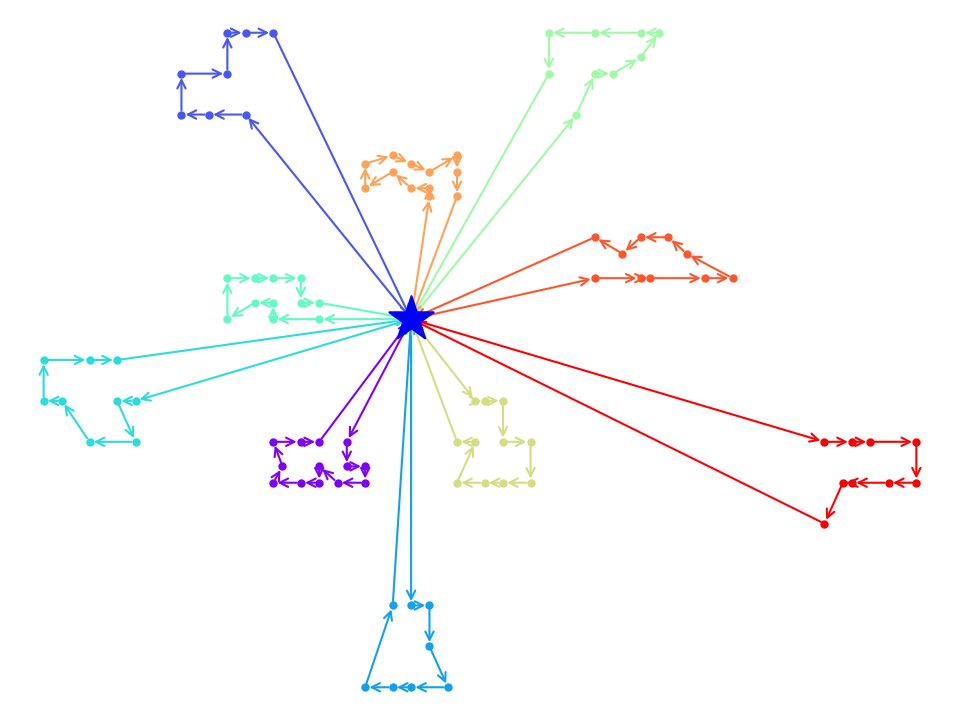
\includegraphics[width=0.6\textwidth]{figures/routes_c101.png} 
        % \includesvg[scale=1]{figures/core-object}
        \caption{VRP với 10 xe phục vụ 100 khách hàng (cấu hình Solomon C101).} 
        % \label{fig:fg_02}
    \end{figure}
\end{frame}

\section{Các nghiên cứu liên quan}
\begin{frame}{Tấn công DNNs - FGM, I-FGM}
    \begin{itemize}
        \item Kí hiệu $\mathbf{x_0}$ và $\mathbf{x}$ lần lượt là mẫu gốc và mẫu đối nghịch,
        $t$ là lớp mục tiêu cần tấn công.

        \item Tấn công dựa trên $L_{\infty}$
        \begin{equation}
            \mathbf{x} = \mathbf{x_0} - \epsilon \times \text{sign}(\nabla J(\mathbf{x_0}, t))
            \label{eq:1}
        \end{equation}
        với $\epsilon$ là độ biến dạng $L_{\infty}$ giữa $\mathbf{x}$ và $\mathbf{x_0}$ và 
        $\text{sign}(\nabla J)$ là dấu của gradient
        
        \item Tấn công dựa trên $L_1$ và $L_2$
        \begin{equation}
            \mathbf{x} = \mathbf{x_0} - \epsilon \frac{\nabla J(\mathbf{x_0}, t)}
            {\lVert \nabla J(\mathbf{x_0}, t) \rVert _q}
            \label{eq:2}
        \end{equation}
        với $q = 1,2$ và $\epsilon$ là độ méo tương quan
    \end{itemize}
\end{frame}

\begin{frame}{Tấn công DNNs - C\&W}
    \begin{itemize}
        \item Thay vì sử dụng hàm mất mát trên tập huấn luyện Carlini và Wagner
        đã thiết kế  một hiệu chỉnh $L_2$ trong hàm mất mát dựa trên lớp logit trong DNNs để sinh 
        ra các mẫu đối nghịch (Carlini and Wagner 2017b)
        \item Công thức này hóa ra là một trường hợp riêng của thuật toát EAD (sẽ được trình bày trong phần sau)
    \end{itemize}
\end{frame}

\begin{frame}{Phòng thủ DNNs}
    \begin{itemize}
        \item Defensive distillation - Chưng cất phòng thủ (Papernot et al.2016b)
        \item Adversarial training - Huấn luyện đối nghịch (Zheng et al. 2016; Madry et al. 2017; 
        Tram`er et al. 2017; Zantedeschi, Nicolae, and Rawat 2017)
        \item Detection methods - Phương pháp dò tìm (Feinman et al. 2017; Grosse et al. 2017; Lu, Issaranon, and Forsyth 2017; 
        Xu, Evans, and Qi 2017)
    \end{itemize}
\end{frame}

\section{EAD: Tấn công Elastic-Net vào DNN}
\begin{frame}{EAD - Tóm lược}
    \begin{itemize}
        \item Hiệu chỉnh elastic-net là công nghệ được sử dụng rộng rãi trong việc giải quyết 
        các bài toán lựa chọn thuộc tính nhiều chiều (Zou and Hastie 2005)

        \item Nhìn chung, hiệu chỉnh elastic-net được sử dụng trong bài toán cực 
        tiểu hóa sau đây:
        \begin{equation}
            \label{eq:3}
            \text{minimize}_{\mathbf{z} \in \mathcal{Z}} \text{ }
            f(\mathbf{z}) + \lambda_1 \lVert \mathbf{z} \rVert_1
            + \lambda_2 \lVert \mathbf{z} \rVert_2^2
        \end{equation}
        Trong đó $\mathbf{z}$ là vector của $p$ biến tối ưu, $\mathcal{Z}$ là tập nghiệm 
        chấp nhận được, $f(\mathbf{z})$ là hàm mất mát, $\lVert \mathbf{z} \rVert_q$ là 
        chuẩn $q$ của $\mathbf{z}$ và $\lambda_1, \lambda_2 \geq 0$ tương ứng là các tham số hiệu 
        chỉnh $L_1$ và $L_2$

        \item Biểu thức $\lambda_1 \lVert \mathbf{z} \rVert_1 + \lambda_2 
        \lVert \mathbf{z} \rVert_2^2$ được gọi là hiệu chỉnh elactic-net của $\mathbf{z}$
    \end{itemize}
\end{frame}

\begin{frame}{EAD - Xây dựng}
    Cho trước 1 ảnh $\mathbf{x_0}$ và nhãn đúng của nó là $t_0$, 
    gọi $\mathbf{x}$ là mẫu đối nghịch của $\mathbf{x_0}$ với lớp đích nhắm đến là $t \neq t_0$ . Hàm mất mát 
    $f(\mathbf{x})$ cho tấn công nhắm đích là:
    \begin{equation}
        \label{eq:4}
        f(\mathbf{x}, t) = \max { \left( \max_{j \neq t} [\textbf{Logit}(\mathbf{x})]_j - 
        [\textbf{Logit}(\mathbf{x})]_t, -\kappa \right) }
    \end{equation}
    Trong đó $\textbf{Logit}(\mathbf{x}) = [\textbf{Logit}(\mathbf{x})_1, ..., 
    \textbf{Logit}(\mathbf{x})_K] 
    \in \mathbb{R}^K$ là lớp logit (lớp trước softmax) biểu diễn cho $\mathbf{x}$ trong mạng DNN, $K$
    là số lượng lớp cần phân loại, $\kappa > 0$ là tham số tin cậy, nó đảm bảo một khoảng 
    cách cố định giữa $\max_{j \neq t} [\textbf{Logit}(\mathbf{x})]_j$ và $[\textbf{Logit}(\mathbf{x})]_t$.
\end{frame}

\begin{frame}{EAD - Xây dựng}
    Thành phần $[\textbf{Logit}(x)]_t$ là xác xuất dự đoán $x$ có nhãn $t$ theo 
    luật phân loại của hàm softmax:
    \begin{equation}
        \label{eq:5}
        \text{Prob}(\text{Label}(\mathbf{x}) = t) = \frac{\exp([\textbf{Logit}(\mathbf{x})]_t)}{
            \sum_{j=1}^{K} \exp([\textbf{Logit}(\mathbf{x})]_j)
        }
    \end{equation}
\end{frame}

\begin{frame}{EAD - Xây dựng}
    Do đó, hàm mất mát trong phương trình (\ref{eq:4}) có mục đích là để cho ra nhãn $t$ là 
    lớp có xác xuất cao nhất của $\mathbf{x}$ và tham số $\kappa$ đảm bảo sự phân biệt giữa lớp $t$
    và lớp dự đoán gần nhất khác với $t$. Với tấn công không nhắm mục tiêu, hàm mất mát trong 
    phương trình \ref{eq:4} trở thành:
    \begin{equation}
        \label{eq:6}\
        f(\mathbf{x}) = \max { \left([\textbf{Logit}(\mathbf{x})]_{t_0} - 
        \max_{j \neq t} [\textbf{Logit}(\mathbf{x})]_j, -\kappa \right) }
    \end{equation}
\end{frame}

\begin{frame}{EAD - Xây dựng}
    Hiệu chỉnh 
    elastic-net còn tạo ra mẫu đối nghịch tương tự với ảnh gốc. Công thức tấn công elastic-net
    vào mạng DNNs (EAD) để tạo ra mẫu đối nghịch $(\mathbf{x},t)$ cho ảnh gốc $(\mathbf{x_0}, t_0)$ như sau:
    \begin{equation}
        \label{eq:7}
        \begin{split}
        &\text{minimize}_{\mathbf{x}} \text{ }
        c \times f(\mathbf{x}, t) + \beta \lVert \mathbf{x} - \mathbf{x_0} \rVert_1
        + \lVert \mathbf{x} - \mathbf{x_0} \rVert_2^2 \\
        &\text{st   } \mathbf{x} \in [0,1]^p
        \end{split}
    \end{equation}
    Với $f(\mathbf{x},t)$ được xác định trong phương trình (\ref{eq:4}), $c, \beta \geq 0$ lần lượt 
    là các tham số  hiệu chỉnh của hàm mất mát $f$ và hàm phạt $L_1$.
\end{frame}

\begin{frame}
    \begin{center}
        \textbf{Thuật toán 1} Tấn công Elastic-net vào DNNs (EAD)
        \begin{itemize}
            \item[] \textbf{Input}: Ảnh gốc và nhãn của nó ($\mathbf{x}_0$, $t_0$), lớp mục tiêu $t$, tham số chuyển giao $\kappa$, tham số hiệu chỉnh $\beta$, độ dài bước $\alpha_k$, số bước lặp $I$
            \item[] \textbf{Output}: mẫu đối nghịch $\mathbf{x}$
            \item[] Khởi tạo: $\mathbf{x}^{(0)}$ = $\mathbf{y}^{(0)}$ = $\mathbf{x}_0$
            \item[] \textbf{for} $k = 0$ to $I - 1$ do
            \begin{itemize}
                \item[] $\mathbf{x}^{(k+1)} = S_{\beta}(\mathbf{y}^{(k)} -\alpha_{k} \nabla g(\mathbf{y}^{(k)}))$
                \item[] $\mathbf{y}^{(k+1)} = \mathbf{x}^{(k+1)} + \frac{k}{k+3} (\mathbf{x}^{(k+1)} - \mathbf{x}^{(k)}) $
            \end{itemize}
            \item[] \textbf{end for}
            \item[] Luật quyết định: tìm $\mathbf{x}$ từ tập các mẫu thành công trong $\{\mathbf{x}^k\}_{k=1}^{I}$ (luật EN, luật $L_1$).
        \end{itemize}
    \end{center}
\end{frame}

\begin{frame}{EAD - Thuật toán}
    Trong đó 
    \begin{equation}
        \label{eq:9}
        [S_{\beta}(\mathbf{z})]_i = 
        \begin{cases}
            \min \{ \mathbf{z}_i - \beta, 1 \} &\text{ nếu } \mathbf{z}_i - \mathbf{x_0}_i  > \beta; \\
            \mathbf{x_0}_i &\text{ nếu } |\mathbf{z}_i - \mathbf{x_0}_i| \leq \beta; \\
            \max \{ \mathbf{z}_i + \beta, 0 \} &\text{ nếu } \mathbf{z}_i - \mathbf{x_0}_i < -\beta
        \end{cases}
    \end{equation}
    Với $i \in \{ 1, ..., p \}$. Nếu $|\mathbf{z}_i - \mathbf{x_0}_i| > \beta$, thành phần 
    $\mathbf{z}_i$ được co lại với hệ số $\beta$ và chiếu thành phần kết quả lên miền ràng buộc 
    chấp nhận được thuộc đoạn $[0,1]$.
\end{frame}

\section{Thực nghiệm}
\begin{frame}{Thực nghiệm: Dữ liệu và phương pháp}
    \begin{itemize}
        \item Tập dữ liệu: MNIST, CIFAR10, ImageNet
        \begin{itemize}
            \item MNIST và CIFAR10 được huấn luyện trên mô hình DNN bởi Carlini và Wagner
            \item ImageNet sử dụng mô hình InceptionV3
        \end{itemize}
        \item Phương pháp tấn công:
        \begin{itemize}
            \item EAD
            \item C\&W
            \item FGM
            \item I-FGM
        \end{itemize}
        \item Phần cứng: Intel E5-2690 v3 CPU, 40 GB RAM, NVIDIA K80 GPU
    \end{itemize}
\end{frame}

\begin{frame}{Thực nghiệm: Độ đo}
    \begin{itemize}
        \item ASR: Tỉ lệ tấn công thành công
        \item $L_1$, $L_2$ và $L_{\infty}$: Các khoảng cách giữa mẫu đối nghịch và ảnh gốc
    \end{itemize}
\end{frame}

\begin{frame}{Thực nghiệm: Các trường hợp quan tâm}
    \begin{itemize}
        \item \textbf{Trường hợp tốt nhất (best case):} tấn công dễ nhất về phương diện nhiễu, trong số các tấn công nhắm tới tất cả các lớp sai nhãn.
        \item \textbf{Trường hợp trung bình (average case):} tấn công nhắm ngẫu nhiên vào 1 lớp sai nhãn.
        \item \textbf{Trường hợp xấu nhất (worst case):} tấn công khó nhất về phương diện nhiễu, trong số những tấn công nhắm tới tất cả các lớp sai nhãn.
    \end{itemize}
\end{frame}

\begin{frame}{Thực nghiệm: Độ nhạy}
    \begin{figure}
        \centering
        \includegraphics[scale=0.5]{images/tab_4_1.png}
    \end{figure}
\end{frame}

\begin{frame}{Thực nghiệm: Luật quyết định}
    \begin{figure}[H] % places figure environment here   
        \centering % Centers Graphic
        \includegraphics[width=1\textwidth]{images/fig_02.png} 
        \caption{So sánh luật quyết định EN và $L_1$ trong EAD trên tập MNIST với nhiều tham số hiệu chỉnh $L_1$ $\beta$ (trường hợp trung bình). So sánh với luật chọn EN tại cùng giá trị $\beta$ thì luật chọn $L_1$ thu được các mẫu ít nhiễu $L_1$ hơn, nhưng đổi lại có thể bị nhiễu $L_2$, $L_{\infty}$ nhiều hơn.}% Creates caption underneath graph
        \label{fig:fg_02}
    \end{figure}
\end{frame}

\begin{frame}{Thực nghiệm: ASR, nhiễu trên MNIST, CIFAR10, ImageNet}
    \begin{figure}
        \centering
        \includegraphics[scale=0.55]{images/tab_4_2.png}
    \end{figure}
\end{frame}

\begin{frame}{Thực nghiệm: MNIST}
    \begin{figure}
        \centering
        \includegraphics[scale=0.2]{images/fig_05.png}
        \caption{Các mẫu đối nghịch được sinh bởi thuật toán EAD trên tập MNIST}% Creates caption underneath graph
        \label{fig:fg_05}
    \end{figure}
\end{frame}

\begin{frame}{Thực nghiệm: CIFAR10}
    \begin{figure}
        \centering
        \includegraphics[scale=0.2]{images/fig_06.png}
        \caption{Các mẫu đối nghịch được sinh bởi thuật toán EAD trên tập CIFAR10}% Creates caption underneath graph
        \label{fig:fg_06}
    \end{figure}
\end{frame}

\begin{frame}{Thực nghiệm: ImageNet}
    \begin{figure}
        \centering
        \includegraphics[scale=0.2]{images/fig_07.png}
        \caption{Các mẫu đối nghịch được sinh bởi thuật toán EAD trên tập ImageNet}% Creates caption underneath graph
        \label{fig:fg_05}
    \end{figure}
\end{frame}
    
\begin{frame}{Thực nghiệm: Phá vỡ chắt lọc phòng thủ}
    \begin{figure}[H] % places figure environment here   
        \centering % Centers Graphic
        \includegraphics[width=0.6\textwidth]{images/fig_3.png} 
        \caption{ASR (trường hợp trung bình) của C\&W và EAD trên tập MNIST và CIFAR10 với các tham số nhiệt $T$ khác nhau cho chắt lọc phòng thủ. Cả 2 phương pháp đều phá vỡ thành công chắt lọc phòng thủ.} % Creates caption  % Creates caption underneath graph
        \label{fig:fg_03}
    \end{figure}
\end{frame}

\begin{frame}{Thực nghiệm: Chuyển giao tấn công}
    \begin{figure}[H] % places figure environment here   
        \centering % Centers Graphic
        \includegraphics[width=0.5\textwidth]{images/fig_04.png} 
        \caption{Khả năng chuyển giao tấn công (trường hợp trung bình) từ mạng không phòng thủ sang mạng chắt lọc phòng thủ  trên tập dữ liệu MNIST với các tham số $\kappa$ khác nhau. EAD có thể đạt ASR gần $99\%$ khi $\kappa = 50$, trong khi ASR lớn nhất của C\&W là gần $88\%$ khi $\kappa=40$.} % Creates caption  % Creates caption underneath graph
        \label{fig:fg_04}
    \end{figure}
\end{frame}

\begin{frame}{Thực nghiệm: Huấn luyện đối nghịch bổ sung}
    \begin{figure}
        \centering
        \includegraphics[scale=0.55]{images/tab_4_3.png}
    \end{figure}
\end{frame}



\section{Nhận xét}
\begin{frame}{Nhận xét: Thời gian tấn công}
    \begin{table}
        \resizebox{\textwidth}{!}{
        \begin{tabular}{l|lllll}
            \hline
            Phương pháp & EAD-EN & FGM-L1 & FGM-L2 & IFGM-L1 & IFGM-L2 \\
            \hline
            Thời gian (s) & 42810 & 893 & 1034 & 3366 &	9922 \\
            \hline
        \end{tabular}} \\
        \caption[Thời gian tính toán]{Thời gian tấn công của các thuật toán trên tập CIFAR10}
        \label{tab:tab_4}
    \end{table}	
    Thời gian tấn công của thuật toán EAD với luật EN là khoảng 11 giờ và gấp khoảng 48 lần khi so sánh với thuật toán nhanh nhất là FGM-L1!
\end{frame}

\begin{frame}{Mở rộng: Thuật toán tổng quát}
    \begin{itemize}
        \item Thuật toán FISTA: cực tiểu hóa hàm $f(\mathbf{x}, t)$ trong phương trình \ref{eq:7}. Để tính được gradient $\nabla g$ ta cần có ràng buộc hàm mất mát của mô hình gốc $f$ phải trơn
        \item Với một hàm $f$ (lồi) bất kì mà không cần ràng buộc về tính trơn của nó. (Shao, Weijia, Fikret Sivrikaya, \& Sahin Albayrak 2022) đã giới thiệu một thuật toán hiệu quả để cực tiểu hóa hàm mục tiêu tổ hợp bằng cập nhật mũ
    \end{itemize}
\end{frame}

\begin{frame}{Mở rộng: Tấn công hệ thống điểm danh GHTK}
    \begin{itemize}
        \item EAD tấn công hệ thống nhận diện bằng khuôn mặt
        \item Tấn công leo thang đặc quyền khi sử dụng khuôn mặt của một nhân viên với quyền thấp hơn để đánh lừa mô hình nhận diện thành một nhân viên với quyền cao hơn
        \item Framework foolbox \footnote{https://github.com/bethgelab/foolbox} đã tích hợp sẵn tấn công EAD và C\&W để sinh ra các mẫu đối nghịch
    \end{itemize}
\end{frame}

\section{Kết luận}
\begin{frame}{Kết luận}
    Nhóm tác giả đã đề xuất mô hình tấn công bằng hiệu chỉnh elastic-net để tạo ra các mẫu đối nghịch trong tấn công DNN. Các kết quả thực nghiệm trên các tập dữ liệu MNIST, CIFAR10 và ImageNet cho thấy các mẫu $L_1$ tạo bởi EAD có thể đạt được tỷ lệ thành công tương đương với các phương pháp tấn công tiên tiến dựa trên $L_2$ và $L_{\infty}$ khi phá vỡ mạng không phòng thủ và phòng thủ chưng cất. Ngoài ra, EAD có thể cải thiện khả năng chuyển giao tấn công và huấn luyện đối nghịch bổ sung. Các kết quả của nhóm tác giả đã chứng minh hiệu quả của EAD và đưa ra hướng mới sử dụng mẫu đối nghịch $L_1$ trong việc huấn luyện đối nghịch và tăng cường an ninh cho DNN.
\end{frame}


% \section*{Tài liệu tham khảo}
% \begin{frame}
%     \frametitle{References}
%     \bibliographystyle{amsalpha}
%     \bibliography{ref.bib}
% \end{frame}
    
\end{document}
